% superimpose command
\makeatletter
\newcommand{\superimpose}[2]{%
	{\ooalign{$#1\@firstoftwo#2$\cr\hfil$#1\@secondoftwo#2$\hfil\cr}}}
\makeatother
% kronecker symmetric
\newcommand{\ostimes}{\circledast}
\renewcommand{\ostimes}{\mathpalette\superimpose{{\otimes}{\ominus}}}
% kronecker a-symmetric
\newcommand{\oatimes}{\circledast}
\renewcommand{\oatimes}{\mathpalette\superimpose{{\otimes}{\varobar}}}

\subsection{Interlude: Box-product and Kronecker-product}

Kronecker-product: $A \otimes B \in \mathbb{R}^{(m_1m_2) \times (n_1n_2)}$ is defined by $(A \otimes B)_{(i - 1)m_2+j,(k - 1)n_2+l} = a_{ik}b_{jl} = (A \otimes B)_{(ij)(kl)}$.

Box-product: $A \boxtimes B \in \mathbb{R}^{(m_1m_2) \times (n_1n_2)}$ is defined by $(A \boxtimes B)_{(i - 1)m_2+j,(k - 1)n_1+l} = a_{il}b_{jk} = (A \boxtimes B)_{(ij)(kl)}$.

I found this box-product only in two sources, one of which is this: \url{https://researcher.watson.ibm.com/researcher/files/us-pederao/ADTalk.pdf} but it generally seems to be very helpful for matrix derivations with transposed matrices.

\subsection{Standard Wishart distribution}

the pdf of the Wishart is

\begin{subequations}
\begin{align}
\mathcal{W}(X; n,p,V) &= \frac{1}{2^{np/2} \left|{\mathbf V}\right|^{n/2} \Gamma_p\left(\frac {n}{2}\right ) }{\left|\mathbf{X}\right|}^{(n-p-1)/2} e^{-(1/2)\operatorname{tr}({\mathbf V}^{-1}\mathbf{X})} \\
&= \exp \left[(n-p-1)/2 \log(|X|) -(1/2)\operatorname{tr}({\mathbf V}^{-1}\mathbf{X}) - \log\left(2^{np/2} \left|{\mathbf V}\right|^{n/2} \Gamma_p\left(\frac {n}{2}\right )\right) \right]\\
&= \frac{1}{X^{\frac{1}{2}}}\exp \left[(n-p)/2 \log(|X|) -(1/2)\operatorname{tr}({\mathbf V}^{-1}\mathbf{X}) - \log\left(2^{np/2} \left|{\mathbf V}\right|^{n/2} \Gamma_p\left(\frac {n}{2}\right )\right) \right]
\end{align}
\end{subequations}

with $h(X) = 1/X^{\frac{1}{2}}$, $\phi(X)=(\log(X), X), w=((n-p)/2, V^{-1})$ and $Z(n,p,V)=\log\left(2^{np/2} \left|{\mathbf V}\right|^{n/2} \Gamma_p\left(\frac {n}{2}\right )\right)$.

\subsubsection{Laplace Approximation of the standard Wishart distribution}

Using $\frac{\partial \det(X)}{\partial X} = \det(X)(X^{-1})^\top$ and $\frac{\partial}{\partial X} Tr(AX) = A^\top$ we can calculate the mode by setting the first derivative of the log-pdf to zero

\begin{align*}
\frac{\partial \log \mathcal{W}(X; n,p,V)}{\partial X} &= \frac{(n-p-1)\det(X)(X^{-\top})}{2\det(X)} - \frac{V^{-\top}}{2} \\
\Rightarrow 0 &= \frac{(n-p-1)X^{-1}}{2} - \frac{V^{-1}}{2} \\
\Leftrightarrow  \frac{(n-p-1)X^{-1}}{2} &= \frac{V^{-1}}{2} \\
\Leftrightarrow X &= (n-p-1)V
\end{align*}

Using the fact that the root of a symmetric matrix is symmetric and $\frac{\partial X^{-1}}{\partial X} = -X^{-1} \otimes X^{-1}$ we get 

\begin{align*}
\frac{\partial^2 \log f(X; n,p,V)}{\partial^2 X} &= -\frac{(n-p-1)}{2} X^{-1} \otimes X^{-1}
\end{align*}

Using $(\alpha A)^{-1} = \alpha^{-1}A^{-1}$, the linearity of the Kronecker product to pull out scalars and $X^{-1} \otimes X^{-1} = (X \otimes X)^{-1}$ to insert the mode and invert we get:

\begin{align*}
-\frac{(n-p-1)}{2} X^{-1} \otimes X^{-1} &= -\frac{(n-p-1)}{2} \frac{1}{(n-p-1)} V^{-1} \otimes \frac{1}{(n-p-1)} V^{-1} \\
&= -\frac{1}{2(n-p-1)}(V \otimes V)^{-1} \\
\Rightarrow \Sigma &= 2(n-p-1)(V \otimes V)
\end{align*}

In summary, the Laplace approximation of a Wishart distribution in the standard basis is $\mathcal{N}\left(X; (n-p-1)V, 2(n-p-1)(V \otimes V)\right)$, where the representation of the symmetric positive definite matrices has been changed from $\mathbb{R}^{n\times n}$ to $\mathbb{R}^{n^2}$.

\subsection{Logm-Transformed Wishart distribution}

we transform the distribution with $g(X) = \text{logm}(X)$, i.e. $X(Y) = g^{-1}(X) = \text{expm}(Y)$, where $\text{expm}(Y)$ is the matrix exponential and $\text{logm}(Y)$ is the matrix logarithm of $Y$. The new pdf becomes

\begin{subequations}
\begin{align}
\mathcal{W}_{\text{logm}}(Y; n, p, V) &= \frac{1}{2^{np/2} \left|{\mathbf V}\right|^{n/2} \Gamma_p\left(\frac {n}{2}\right ) }{\left|\mathbf{\operatorname{expm}Y}\right|}^{(n-p-1)/2} e^{-(1/2)\operatorname{tr}({\mathbf V}^{-1}\mathbf{\operatorname{expm}Y})} \cdot |\operatorname{expm}Y| \\ 
&= \frac{1}{2^{np/2} \left|{\mathbf V}\right|^{n/2} \Gamma_p\left(\frac {n}{2}\right ) }{\left|\mathbf{\operatorname{expm}Y}\right|}^{(n-p+1)/2} e^{-(1/2)\operatorname{tr}({\mathbf V}^{-1}\mathbf{\operatorname{expm}Y})} \\ 
&= \exp \left[C + \frac{(n-p+1)}{2} \log(\left|\mathbf{\operatorname{expm}Y}\right|)  - \frac{1}{2}\operatorname{tr}({\mathbf V}^{-1}\mathbf{\operatorname{expm}Y}) \right]
\end{align}
\end{subequations}

with $h(Y) = Y^{\frac{1}{2}}, \phi(Y) = (Y, \operatorname{expm}Y), w = (n-p), V^{-1}$ and $Z(n,p,V)=\log\left(2^{np/2} \left|{\mathbf V}\right|^{n/2} \Gamma_p\left(\frac {n}{2}\right )\right)$.

\subsubsection{Laplace Approximation of the logm-transformed Wishart distribution}

To compute the first derivative we use the following

\begin{align}
	\frac{\partial \log(\det(\operatorname{expm}(Y)))}{\partial Y} 
	&= \frac{\partial \log(\det(\operatorname{expm}(Y)))}{\partial \det(\operatorname{expm}(Y))} \cdot \frac{\partial \det(\operatorname{expm}(Y))}{\partial \operatorname{expm}(Y)} \cdot \frac{\partial \operatorname{expm}(Y)}{\partial Y} \\
	&= \frac{1}{\det(\operatorname{expm}(Y))} \cdot \det(\operatorname{expm}(Y)) \operatorname{expm}(Y)^{-\top} \cdot \operatorname{expm}(Y) \\
	&= I_p
\end{align}

where $I_p$ is the identity matrix of size $p$ and we use the fact that the matrix logaritm of a symmetric matrix is symmetric, implying $\operatorname{expm}(Y)^{-\top} = \operatorname{expm}(Y)^{-1}$. With this we get the first derivative

\begin{subequations}
\begin{align}
	\frac{\partial \log W_{log}}{\partial Y} &= \frac{\partial}{\partial Y} \left[C + \frac{(n-p+1)}{2} \log(\left|\mathbf{\operatorname{expm}Y}\right|)  - \frac{1}{2}\operatorname{tr}({\mathbf V}^{-1}\mathbf{\operatorname{expm}Y}) \right] \\
	&=  \frac{(n-p+1)}{2} I_p - \frac{1}{2}V^{-1}\mathbf{\operatorname{expm}Y} 
\end{align}
\end{subequations}

By setting this to zero we get a mode of

\begin{subequations}
\begin{align}
	0 &=  \frac{(n-p+1)}{2} I_p - \frac{1}{2}V^{-1}\mathbf{\operatorname{expm}Y} \\
	\Leftrightarrow (n-p+1)I_p &= V^{-1}\mathbf{\operatorname{expm}Y} \\
	\Leftrightarrow Y &= \operatorname{logm}((n-p+1)V)
\end{align}
\end{subequations}

For the second derivative we use the fact that

\begin{subequations}
\begin{align}
	\frac{\partial (B\operatorname{expm}(Y))_{kl}}{\partial Y_{ij}} &= \delta_{jl}(B\operatorname{exmp}(Y))_{ki} \\
	\Leftrightarrow \frac{\partial B\operatorname{expm}(Y)}{\partial Y} &= \left(B\operatorname{expm}(Y) \otimes I_p\right)
\end{align}
\end{subequations}

yielding

\begin{subequations}
\begin{align}
	\frac{\partial^2 \log \mathcal{W}_{\text{logm}}}{\partial^2 Y} &= \frac{\partial \log \mathcal{W}_{\text{logm}}}{\partial Y}  \frac{(n-p+1)}{2} I_p - \frac{1}{2}V^{-1}\mathbf{\operatorname{expm}Y} \\
	&= -\frac{1}{2}(V^{-1}\mathbf{\operatorname{expm}Y} \otimes I_p) \\
	&\overset{\text{mode}}{\Rightarrow} -\frac{1}{2}((n-p+1)V^{-1}V \otimes I_p) \\
	&= -\frac{(n-p+1)}{2} (I_p \otimes I_p)\\
	\Leftrightarrow \Sigma &= \frac{2}{n-p+1} I_{p^2}
\end{align}
\end{subequations}

where $I_{p^2}$ is an Identity matrix of size $p^2$. 

\subsubsection{The Bridge for logm-tranform}

$\mu$ and $\Sigma$ are already given by the Laplace approximation. Inverting the mode yields an estimate for $V$. 

\begin{align}
	\mu &= \operatorname{logm}((n-p+1)V) \Leftrightarrow \operatorname{expm}(\mu) = (n-p+1)V \Leftrightarrow V = \frac{\operatorname{expm}(\mu)}{(n-p+1)}
\end{align}

where $\mu$ and $V$ are reshaped to a matrix of size $p\times p$. In summary this yields

\begin{subequations}
\begin{align}
	\mu &= \operatorname{logm}((n-p+1)V) \\
	\Sigma &= \frac{2}{n-p+1} I_{p^2} \\
	V &= \frac{\operatorname{expm}(\mu)}{(n-p+1)} \\
	n &= ?
\end{align} 
\end{subequations}

\subsection{Sqrtm-Transformed Wishart distribution}

we transform the distribution with $g(X) = \text{sqrtm}(X) = X^{\frac{1}{2}}$, i.e. $X(Y) = g^{-1}(X) = Y^2$, where $\text{sqrtm}(Y)$ is the square root of the matrix. The new pdf becomes

\begin{subequations}
\begin{align}
\mathcal{W}_{\text{sqrm}}(Y; n,p,V) &= \frac{1}{2^{np/2} \left|{\mathbf V}\right|^{n/2} \Gamma_p\left(\frac {n}{2}\right ) }{\left|\mathbf{Y^2}\right|}^{(n-p-1)/2} e^{-(1/2)\operatorname{tr}({\mathbf V}^{-1}\mathbf{Y^2})} \cdot |2Y| \\ 
&= \frac{1}{2^{np/2} \left|{\mathbf V}\right|^{n/2} \Gamma_p\left(\frac {n}{2}\right ) }{\left|\mathbf{Y}\right|}^{2(n-p-1)/2} e^{-(1/2)\operatorname{tr}({\mathbf V}^{-1}\mathbf{Y^2})} \cdot 2^p|Y| \\
&= \frac{1}{2^{np/2} \left|{\mathbf V}\right|^{n/2} \Gamma_p\left(\frac {n}{2}\right ) }{\left|\mathbf{Y}\right|}^{(n-p)} e^{-(1/2)\operatorname{tr}({\mathbf V}^{-1}\mathbf{Y^2})} \\
&= \exp \left[(n-p) \log(|Y|) - (1/2)\operatorname{tr}({\mathbf V}^{-1}\mathbf{Y^2}) - \log\left(2^{np/2} \left|{\mathbf V}\right|^{n/2} \Gamma_p\left(\frac {n}{2}\right )\right)\right]
\end{align}
\end{subequations}

with $h(Y) = 1, \phi(Y)=(\log(Y), Y^2), \eta=((n-p), V^{-1})$ and $Z(n,p,V)=\log\left(2^{np/2} \left|{\mathbf V}\right|^{n/2} \Gamma_p\left(\frac {n}{2}\right )\right)$. 
We drop the $2^p$ because there are $2^p$ matrices that are a root of $X$ as already explained in subsection TODO. 

\subsubsection{Laplace Approximation of the sqrtm-transformed Wishart distribution}

Using $\frac{\partial \det(Y)}{\partial Y} = \det(Y)(Y^{-1})^\top$ and $\frac{\partial}{\partial Y} Tr(AY^2) = (AY + YA)^T$ we can calculate the mode by setting the first derivative of the log-pdf to zero

\begin{subequations}
\begin{align}
\frac{\partial \log \mathcal{W}_{\text{sqrtm}}(Y; n,p,V)}{\partial Y} &= \frac{(n-p)\det(Y)(Y^{-\top})}{\det(Y)} - \frac{(V^{-1}Y + YV^{-1})^\top}{2} \\
\Rightarrow 0 &= (n-p)Y^{-\top} - \frac{(V^{-1}Y + YV^{-1})^\top}{2} \\
\Leftrightarrow  (n-p)Y^{-\top} &=  \frac{(V^{-1}Y + YV^{-1})^\top}{2} \\
\Leftrightarrow  (n-p)Y^{-1} &=  \frac{(V^{-1}Y + YV^{-1})}{2} \\
\Leftrightarrow Y &= ???
\end{align}
\end{subequations}

THIS IS WHERE SOLVING FOR Y GETS COMPLICATED. Maybe we can rewrite it with Kronecker products and vectorized matrices like for the Sylvester equation and these laws \url{https://en.wikipedia.org/wiki/Vectorization_(mathematics)#Compatibility_with_Kronecker_products}.

So far I have found the following relationships that don't get me any further to the solution of $Y$:

\begin{align*}
(n-p)Y^{-1} &=  \frac{(V^{-1}Y + YV^{-1})}{2} \\
\Leftrightarrow C &= BY + YBY \\
\Leftrightarrow C &= (I_p \otimes BY)\vec{Y} + (B^TY^T \otimes I_p)\vec{Y} \\
\Leftrightarrow C &= (B^TY^T \oplus BY)\vec{Y} \\
\Leftrightarrow C &= (BY \oplus BY)\vec{Y}
\end{align*}

Computing the second derivative by using $\frac{\partial}{\partial Y}Y^{-1} = -Y^{-1} \otimes Y^{-1}$, $\frac{\partial}{\partial Y} (AY + YA)^\top = I \boxtimes A + A \boxtimes I$. For simplicity we approximate the mode with $Y = \sqrt{(n-p)V}$. 

\begin{subequations}
\begin{align}
\frac{\partial^2 \log \mathcal{W}_{\text{sqrtm}}(Y; n,p,V)}{\partial^2 Y} &= \frac{\partial}{\partial Y} \left[(n-p)Y^{-\top} - \frac{(V^{-1}Y + YV^{-1})^\top}{2}\right] \\
&= -(n-p) (Y^{-\top} \otimes Y^{-1}) + \frac{1}{2}(I_p \boxtimes V^{-1} + V^{-1} \boxtimes I_p) \\
&\overset{\text{mode}}{\Rightarrow} -(n-p) \left[\sqrt{\frac{1}{(n-p)}}V^{-\frac{1}{2}} \otimes \sqrt{\frac{1}{(n-p)}}V^{-\frac{1}{2}}\right] + \frac{1}{2}\left[I_p \boxtimes V^{-1} + V^{-1} \boxtimes I_p\right] \\
&= - \left(V^{-\frac{1}{2}} \otimes V^{-1}\right) + \frac{1}{2}\left[I_p \boxtimes V^{-1} + V^{-1} \boxtimes I_p\right] \\
&\overset{\cdot -1}{\Rightarrow} \left(V^{-\frac{1}{2}} \otimes V^{-\frac{1}{2}}\right) - \frac{1}{2}\left[I_p \boxtimes V^{-1} + V^{-1} \boxtimes I_p\right] \\
\Rightarrow \Sigma &= \left[V^{-\frac{1}{2}} \otimes V^{-\frac{1}{2}} - \frac{1}{2}\left(I_p \boxtimes V^{-1} + V^{-1} \boxtimes I_p\right)\right]^{-1} \\
\end{align}
\end{subequations}

We can assume that $Y$ is symmetric because the root of a symmetric positive definite matrix is symmetric. 
This is the solution ONLY if we assume that the mode is given by $Y = \sqrt{(n-p)}V^{\frac{1}{2}}$. 

\subsubsection{The Bridge for sqrtm-tranform}

we use $\mu =  ((n-p)V)^{\frac{1}{2}} \Leftrightarrow \mu^2 = (n-p)V \Leftrightarrow V = \frac{\mu^2}{(n-p)}$. Remember that $\mu$ is reshaped to be the same size as $V$ even though we usually think of it in vector-form. 

\begin{subequations}
\begin{align}
	\mu &=  ((n-p)V)^{\frac{1}{2}} \\
	\Sigma &= \left[V^{-\frac{1}{2}} \otimes V^{-\frac{1}{2}} - \frac{1}{2}\left(I_p \boxtimes V^{-1} + V^{-1} \boxtimes I_p\right)\right]^{-1} \\
	V &= \frac{\mu^2}{(n-p)} \\
	n &= ?
\end{align}
\end{subequations}

STRUGGLE: how to get $n$?  \\
INTERESTING: choosing $\Sigma = 1/4 \cdot (V^{\frac{1}{2}} \ostimes V^{\frac{1}{2}}) $ also yields pretty good results.

\begin{figure}[!htb]
	\centering
	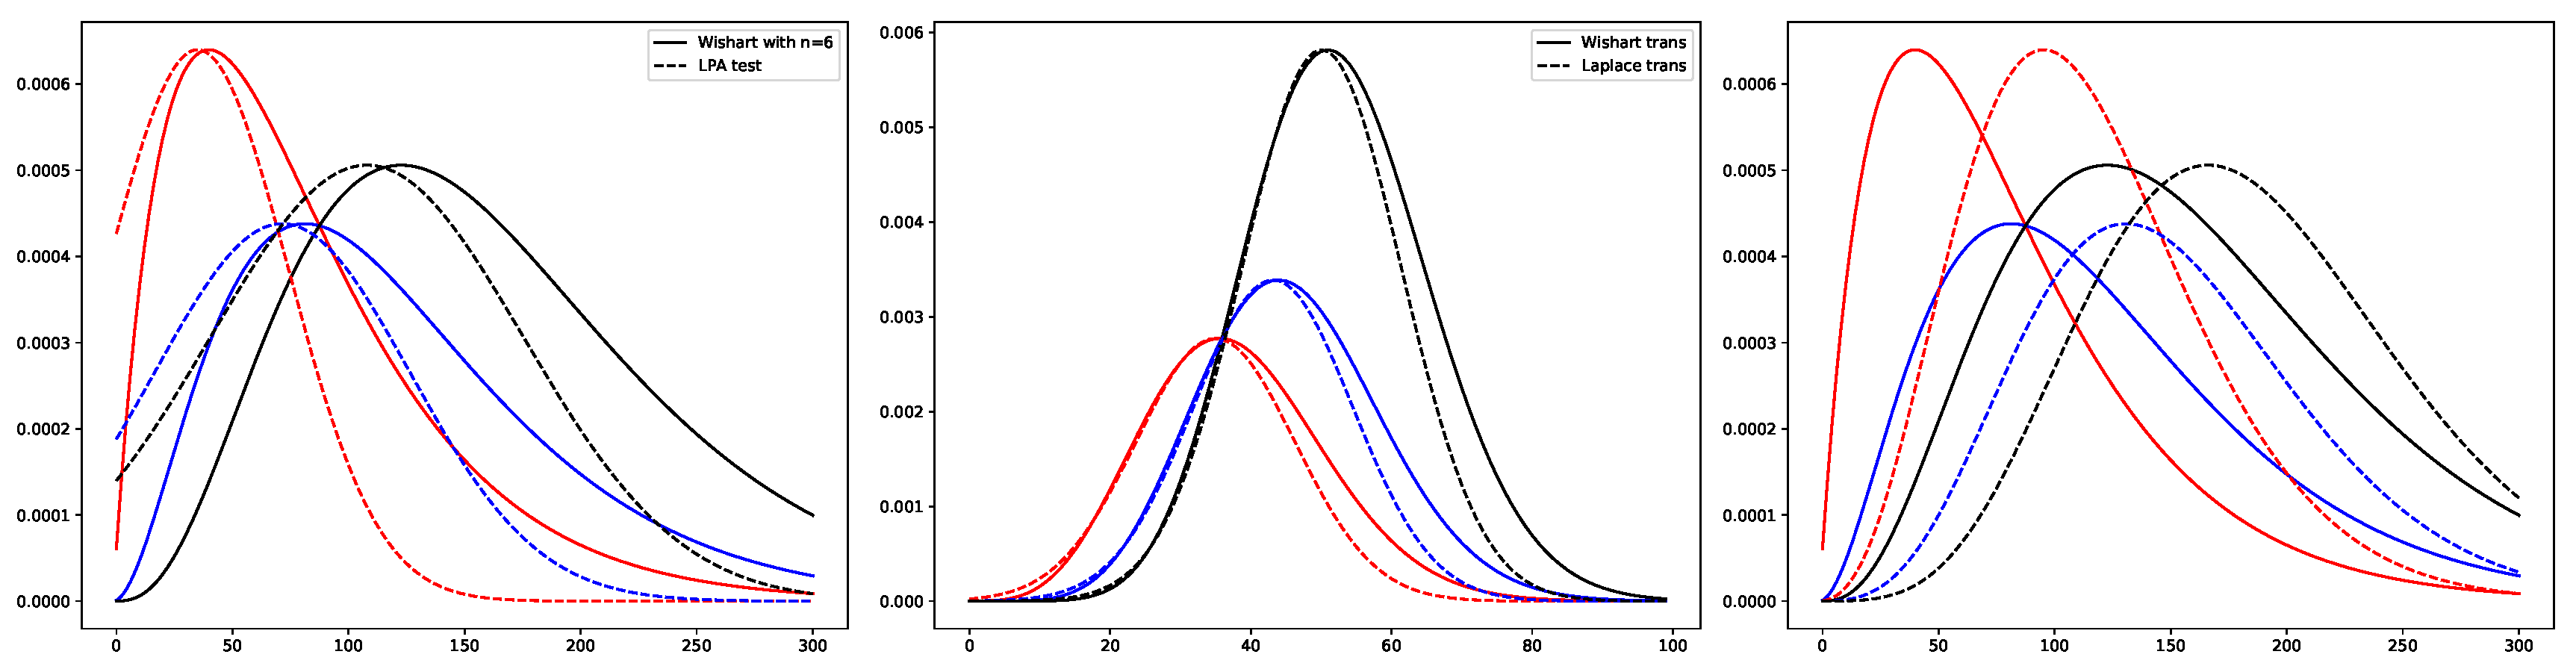
\includegraphics[width=\textwidth]{figures/wishart_sqrtm_bridge.pdf}
	\caption{wishart comparison for sqrtm}
	\label{fig:wishart_comparison}
\end{figure}




